\documentclass[tikz]{standalone}
\usepackage{bm}
\begin{document}
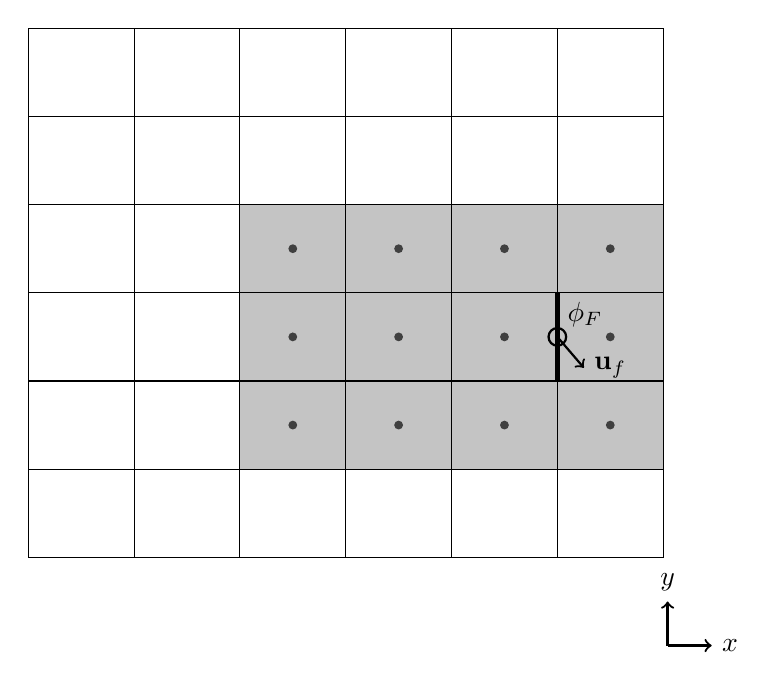
\begin{tikzpicture}[
  scale=0.56,
  cpnt/.style={fill=black!75},
]
\definecolor{stencil}{RGB}{196,196,196}

\draw [thick, ->] (14.5,-2) -- (14.5,-1) node [at end, anchor=south] {$y$};
\draw [thick, ->] (14.5,-2) -- (15.5,-2) node [at end, anchor=west] {$x$};

\begin{scope}[shift={(4.8,2)}]
\fill [stencil] (0,0) rectangle (9.6,6);
\end{scope}

\draw (0,0) rectangle (14.4,12);
\draw (0,2) -- (14.4,2);
\draw (0,4) -- (14.4,4);
\draw (0,6) -- (14.4,6);
\draw (0,8) -- (14.4,8);
\draw (0,10) -- (14.4,10);

\draw (0,0) -- (0,12);
\draw (2.4,0) -- (2.4,12);
\draw (4.8,0) -- (4.8,12);
\draw (7.2,0) -- (7.2,12);
\draw (9.6,0) -- (9.6,12);
\draw (12,0) -- (12,12);


\begin{scope}[shift={(4.8,2)}]
\draw [ultra thick] (7.2,2) -- (7.2,4);
\draw [thick] (7.2,3) circle [radius=0.2] node [anchor=south west] {$\phi_F$};
\draw [thick, ->] (7.2,3) -- (7.8,2.3) node [anchor=west] {$\mathbf{u}_f$};

\path [cpnt] (1.2,1) circle [radius=0.1];
\path [cpnt] (1.2,3) circle [radius=0.1];
\path [cpnt] (1.2,5) circle [radius=0.1];

\path [cpnt] (3.6,1) circle [radius=0.1];
\path [cpnt] (3.6,3) circle [radius=0.1];
\path [cpnt] (3.6,5) circle [radius=0.1];

\path [cpnt] (6.0,1) circle [radius=0.1];
\path [cpnt] (6.0,3) circle [radius=0.1];
\path [cpnt] (6.0,5) circle [radius=0.1];

\path [cpnt] (8.4,1) circle [radius=0.1];
\path [cpnt] (8.4,3) circle [radius=0.1];
\path [cpnt] (8.4,5) circle [radius=0.1];
\end{scope}

\end{tikzpicture}
\end{document}
